\chapter{Outils d'analyse de défauts fonctionnels ESD}
\label{chap:4}

Jusqu'à présent, l'étude s'est focalisée sur le développement de méthodes pour l'acquisition de données de mesures.
Ces mesures nécessitent la réalisation du circuit intégré afin de pouvoir le tester.
Ce procédé est couteux et intervient tard dans le flot de conception.
Les outils de simulation en revanche sont utilisables dés le début du flot de conception.
Ils peuvent donc largement compléter les systèmes de mesures présentés dans le chapitre précédent.
Dans ce chapitre-ci, deux méthodes différentes sont présentes.
La première est destinée aux concepteurs de circuits intégrés, tandis que la seconde vise plutôt les équipementiers.

\section{Méthode bottom-up}

% What is bottom up
L'approche présentée ici est apellée bottom-up, c'est à dire du bas vers le haut.
Elle consiste à caractériser de petites fonctions assez bas dans la hiérarchie du circuit intégré, de manière individuelle, puis d'assembler ensemble leurs modèles afin de déduire le comportement global.
Cett approche présente l'intérêt que des fonctions individuelles sont susceptibles d'être réutilisées, et donc que l'effort de charactérisation et de modélisation n'a besoin d'être fourni qu'une seule fois.
Un schéma de charactérisation assez simple est utilisé en simulation pour charactériser chaque bloc (Fig. \ref{block_function_cz}).
Il fournit l'alimentation nécessaire à la fonction qui doit être en fonctionnement.
Il permet également d'injecter sur une entrée un stress électrique et d'observer la réponse sur une sortie.

\begin{figure}[!h]
  \centering
  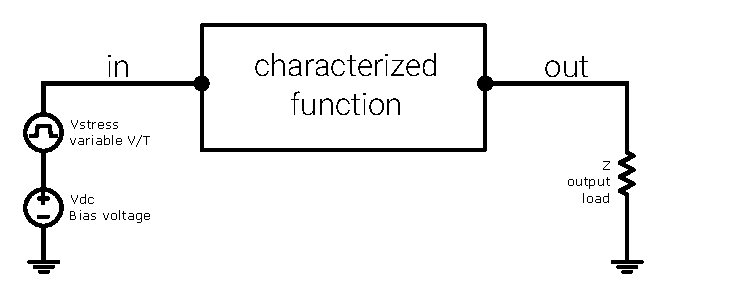
\includegraphics{src/1/figures/characterization_setup.pdf}
  \caption{Block characterization setup (supply input)}
  \label{block_function_cz}
\end{figure}

% What are the characterization signal
%TODO ref
Le signal de charactérisation est une impulsion rectangulaire, appliquée sur l'entrée sous test.
Un ensemble de simulations est effectué en faisant varier les paramètres de cette forme d'onde, injectée sur l'entrée.
Plus précisément, une analyse paramétrique est réalisée sur l'amplitude et la durée de l'impulsion.
Cet ensemble de simulations est résumé dans la Fig. \ref{set_input_signals}.
Cette méthode de charactérisation est fortement inspirée de la méthode Wunsch & Bell \cite{}.

%TODO: Fix sim 12 sim12
\begin{figure}[!h]
  \centering
  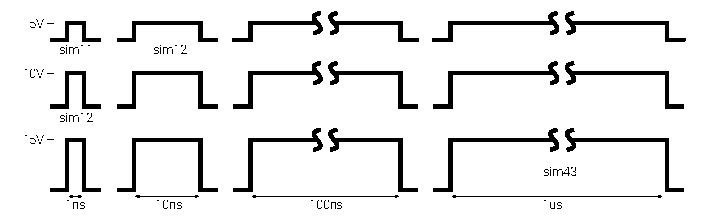
\includegraphics{src/1/figures/time_domain_cz_curves.pdf}
  \caption{Variations on (amplitude, duration) of the input characterization signal}
  \label{set_input_signals}
\end{figure}

Une fois chaque signal injecté, la sortie est observée.
Deux paramètres sont extraits de la forme d'onde de sortie.
L'amplitude maximale est extraite, correspondant à la plus large variation de tension par rapport à un niveau nominal.
La durée de cette variation, à 90\% de l'amplitude maximale est aussi relevée.
Ces deux paramètres permettent de décrire une boite englobante de la forme d'onde de sortie, constituant une sorte de forme d'onde simplifiée.
Cette analyse est effectuée pour chaque simulation.

Il en résulte deux tables, la première associant constituant le modèle du bloc.
La première table associes aux deux paramètres d'entrée (amplitude et durée) une amplitude maximale de sortie.
La seconde table associe aux deux paramètres d'entrée une durée de sortie.
Ces deux tables peuvent ensuite être intégrées dans un modèle, décrit Fig. \ref{fig:principle-transfert-func-v2}.
La fonction $F_{W}$ utilises la première table, pour retourner une amplitude de sortie en fonction des paramètres d'entrée.
La fonction $F_{V}$ utilises la seconde table et retourne une durée.
Sachant que ce modèle accepte les mêmes types de paramètres en entrée et en sortie, plusieurs modèles peuvent être chaînés les uns à la suite des autres, afin de reconstituer le comportement d'une fonction haut-niveau.

\begin{figure}[!h]
  \centering
  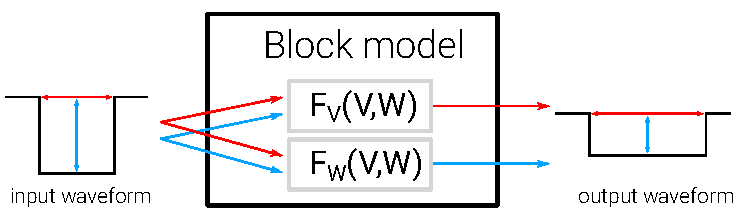
\includegraphics{src/1/figures/principle_transfert_function_v2.pdf}
  \caption{Improved modelling method}
  \label{fig:principle-transfert-func-v2}
\end{figure}

% First run the reference sim
Pour tester cette approche, des simulations sont effectuées en utilisant les schémas Fig. \ref{fig:hypothesis-setup}.
L'objectif est de comparer une simulation transistor de la fonction globale, à une chaine de simulation individuelle de blocs, pour vérifier si des réponses similaires peuvent être obtenues sur la broche de sortie lorsque la broche d'entrée est exposée au même stimuli.

\begin{figure}[!h]
  \centering
  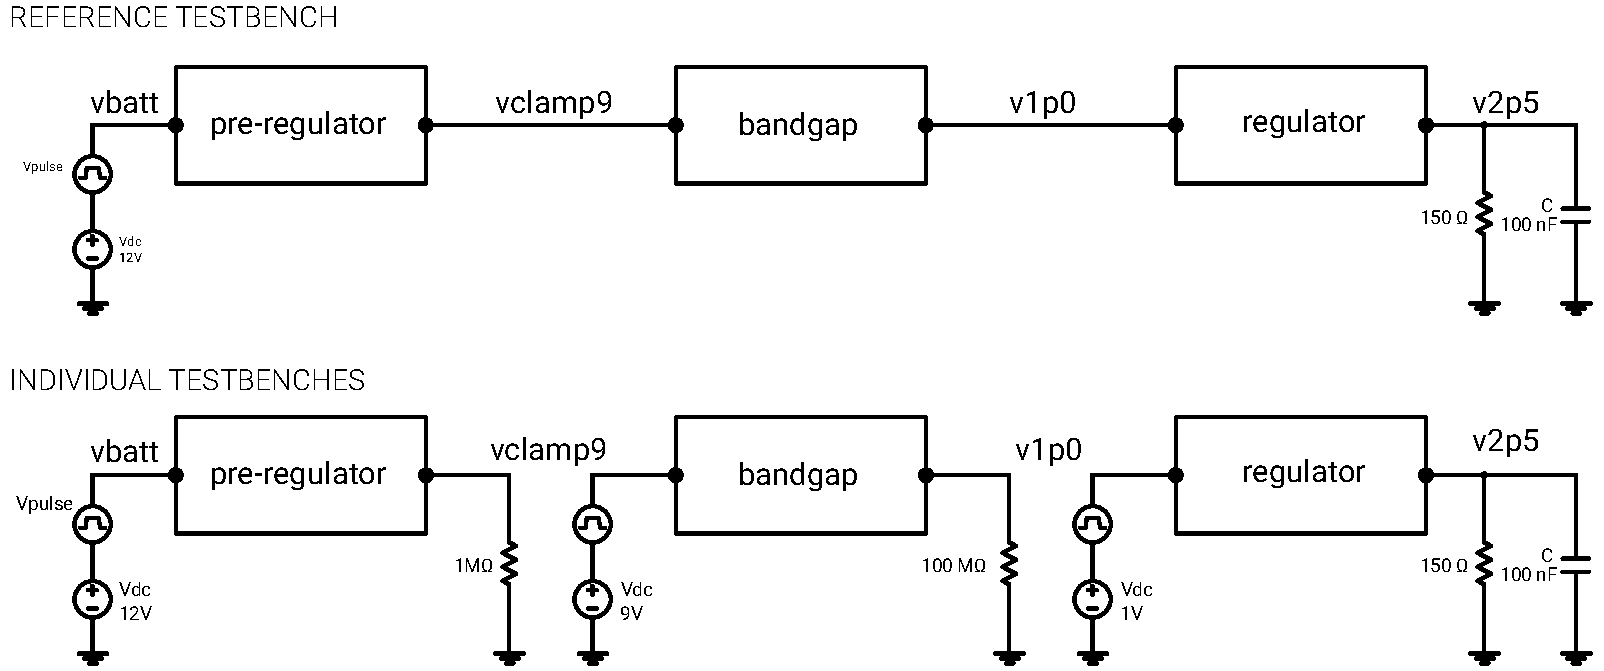
\includegraphics[width=0.98\textwidth]{src/1/figures/hypothesis_testing_setup.pdf}
  \caption{Testbenches used for characterization and hypothesis testing}
  \label{fig:hypothesis-setup}
\end{figure}

% Then do the same thing but with the individual models
La courbe du pré-régulateur seul est donnée Fig. \ref{fig:sim-compare-block1} et comparée avec la simulation totale.
Les deux courbes sont plutôt similaires.
La sortie est estimée avoir une amplitude maximale de -1.5 V (les stress sont d'amplitude négative) et une durée de 880 ns.
Ces deux valeurs sont utilisées comme paramètres d'entrée sur le second modèle, celui du bandgap.

\begin{figure}[!h]
  \centering
  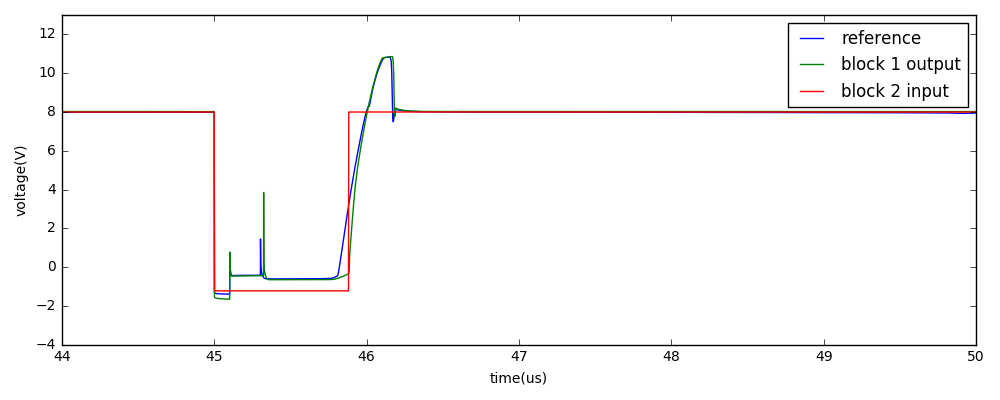
\includegraphics[width=0.98\textwidth]{src/1/figures/simulation_comparison_block1.png}
  \caption{$V_{clamp9}$ waveform}
  \label{fig:sim-compare-block1}
\end{figure}

% Second block output
A la sortie du second block, des différences plus larges apparaissent entre la simulation individuelle et totale. (Fig. \ref{fig:sim-compare-block2}).
La courbe verte a une pente plus longue que la référence.
Néanmoins, les courbes ont quand même des charactéristiques communes en terme d'amplitude maximale et de durée, ce qui est intéressant en regard de cette méthode de modélisation.
La courbe de sortie est analysée et son amplitude maximale déterminée à 0V avec une durée de 2 \textmugreek{}s.
Ces deux valeurs sont appliquées sur l'entrée de la troisième simulation.

\begin{figure}[!h]
  \centering
  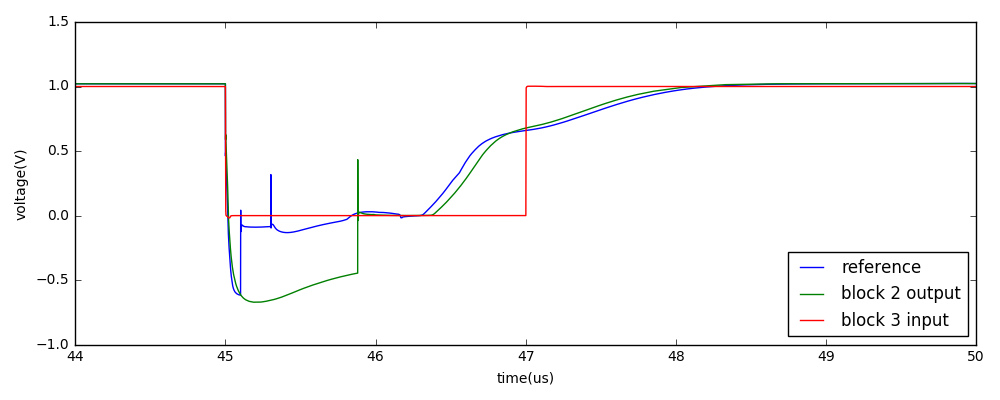
\includegraphics[width=0.98\textwidth]{src/1/figures/simulation_comparison_block2.png}
  \caption{$V_{1p0}$ waveform}
  \label{fig:sim-compare-block2}
\end{figure}

% Third output
A la sortie du dernier bloc, (Fig. \ref{fig:sim-compare-block3}), les deux formes d'onde sont similaires.
La différence d'amplitude maximale est due à un offset aussi présent en statique, et pouvant donc être aisément corrigé.
La courbe de référence est retardée par rapport à la courbe individuelle, mais sinon les deux courbes se ressemblent énormément.

\begin{figure}[!h]
  \centering
  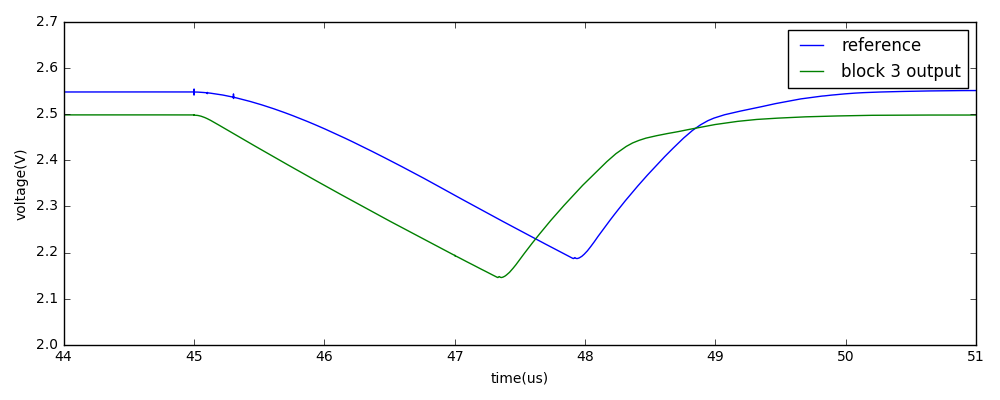
\includegraphics[width=0.98\textwidth]{src/1/figures/simulation_comparison_block3.png}
  \caption{$V_{2p5}$ waveform}
  \label{fig:sim-compare-block3}
\end{figure}

% Conclusion, it works for this case
En conclusion, pour ce cas d'étude, la méthode de simulation et modélisation individuelle aurait permit, par chainage des modèles d'estimer correctement la perturbation sur le bloc de sortie.
Avant de pouvoir généraliser son utilisation, il serait nécessaire de tester cette méthode sur une plus large gamme d'applications.
Elle montre néanmoins des résultats prometteurs.

\section{Méthode boite noire}

% Difference with bottom-up, not the same application, not the same goal
La méthode boite noire exposée ci-après a pour but de modéliser une fonction d'un circuit intégré, entre une entrée et une sortie.
L'objectif est d'effectuer une simulation ESD au niveau carte électronique, pendant le fonctionnement normal, en prenant en compte les circuits intégré.
Cette méthode nécessite de charactériser la fonction de transfert d'une fonction intégrée sur silicium, entre une broche d'entrée et une broche de sortie toutes deux externes.

% introduction, failure relation between input and output
Le principal avantage de cette méthode est de s'abstraire au niveau système de la complexité au niveau circuit intégré.
La charactérisation est effectuée en appliquant une fois de plus une impulsion rectangulaire d'amplitude et de durée variables.
La broche d'entrée reçoit ce stress, pendant que la broche de sortie est surveillée et mesurée.

% What is characterized
Pour tester cette méthode, elle est appliquée en simulation sur la schématique du véhicule de test détaillé dans le chapitre 3.
Les impulsions de charactérisation sont injectées sur l'entrée $V_{batt}$.
La broche de sortie à surveiller est la pin $V_{2p5}$, correspondant à l'alimentation 2.5V régulée.
Un seuil à 2.1V est fixé en dessous duquel une défaillance est considérée.
En dessous de ce seuil, les portes logiques ne sont plus garanties de fonctionner correctement.
La figure \ref{fig:cz-black-box} affiche la présence d'une faute en fonction des paramètres du stress d'entrée.
L'axe des abscisses correspond à la largeur d'impulsion, et celui des ordonnées à l'amplitude du stress.
En soi, cette courbe peut être utilisée dans une simulation comme modèle de faute du bloc.
Avec une largeur d'impulsion et une amplitude appliquée sur $V_{batt}$, la courbe permet d'estimer ou non la présence d'une faute sur la sortie.

\begin{figure}[!h]
  \centering
  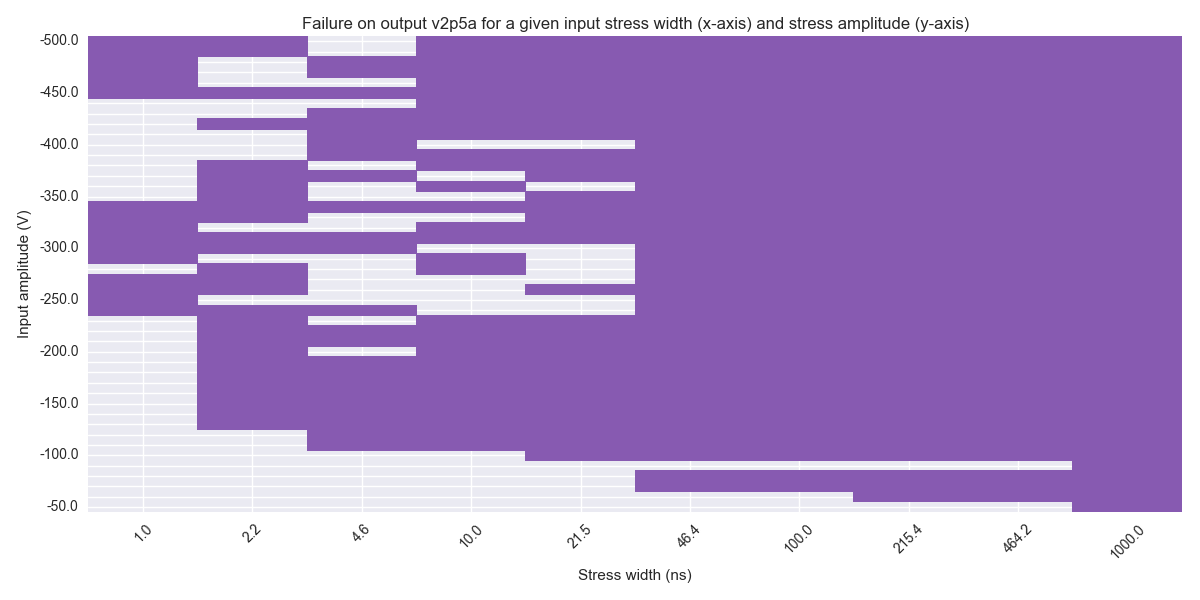
\includegraphics[width=\textwidth]{src/1/figures/black_box_regulator.png}
  \caption{Black-box characterization of the regulation function}
  \label{fig:cz-black-box}
\end{figure}

% What to do with that
Néanmoins, l'objectif final de la méthode boite noire est aussi de fournir un modèle électrique équivalent du circuit intégré.
Le modèle de faute n'est pas un modèle électrique, et ne permet pas de déterminer par exemple pour une tension donnée quel couran est absorbé par une broche.
Par conséquent, il est aussi nécessaire de développer un modèle électrique équivalent de la broche.
Afin d'extraire un modèle I(V), des charactérisations sont effectuées avec la méthode TLP en simulation.
La charactérisation est effectuée à la fois sur un circuit alimenté et non alimenté.
L'objectif est de déterminer l'impact de l'alimentation sur la courbe TLP.
Les charactérisations de l'entrée et de la sortie dans les deux conditions d'alimentation sont fournies dans les figures \ref{fig:tlp-input-cz} et \ref{fig:tlp-output-cz}.

\begin{figure}[!h]
  \centering
  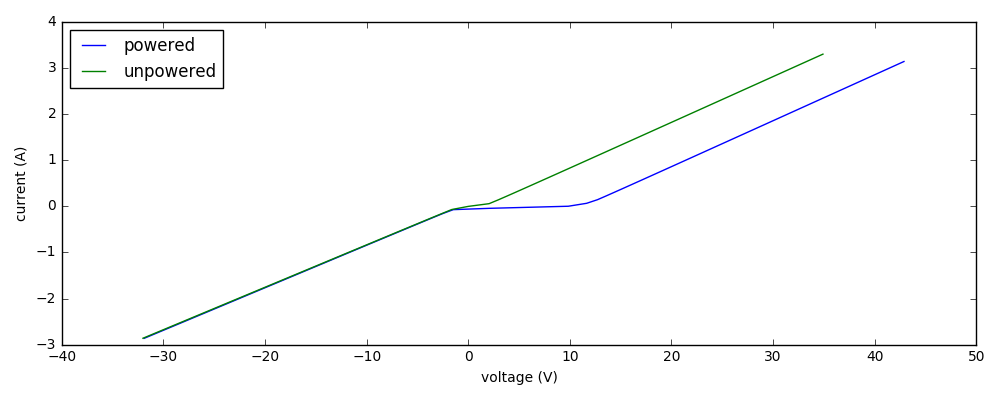
\includegraphics[width=\textwidth]{src/1/figures/tlp_input_characterization.png}
  \caption{TLP characterization of function input in powered and unpowered conditions}
  \label{fig:tlp-input-cz}
\end{figure}

\begin{figure}[!h]
  \centering
  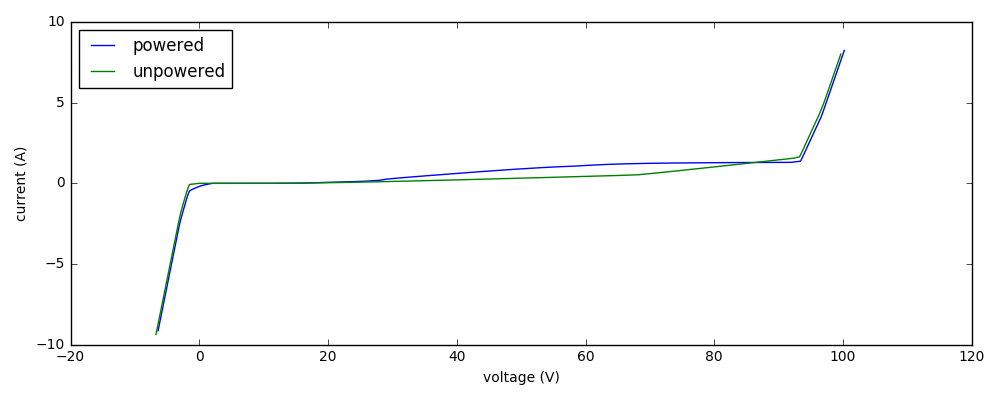
\includegraphics[width=\textwidth]{src/1/figures/tlp_output_characterization.png}
  \caption{TLP characterization of function output in powered and unpowered conditions}
  \label{fig:tlp-output-cz}
\end{figure}

Pour l'entrée et la sortie, de grandes différences sont observées entre un circuit alimenté et non alimenté.
Des quantités différentes de courant sont absorbées par le circuit dans chaque condition.
Puisque le modèle est destiné à des simulations du composant en fonctionnement, la charactérisation en alimenté est selectionnée par la suite.

% Explain the PWL model
Maintenant que le circuit est charactérisé, il est possible d'en construire un modèle électrique.
La stratégie utilisée est de reproduire la courbe I(V) avec une courbe linéaire par morceaux, en utilisant le language de description matérielle Verilog-A.
Le code source du modèle est fourni dans le document complet.
% Validate the model with TLP
Le modèle est construit pour la broche d'entrée puis simulé et comparé à la schématique complète.
Il a été vérifié pour un amplitude de stress de -10V (Fig. \ref{fig:compare-model-simu-m10}, Fig. \ref{fig:compare-model-simu-20}, Fig. \ref{fig:compare-model-simu-40}).
D'autres validations à 20V et 40V sont fournies dans le document complet.
Globablement, une bonne corrélation entre le modèle et le circuit complet est observée pour l'entrée.

\begin{figure}[!h]
  \centering
  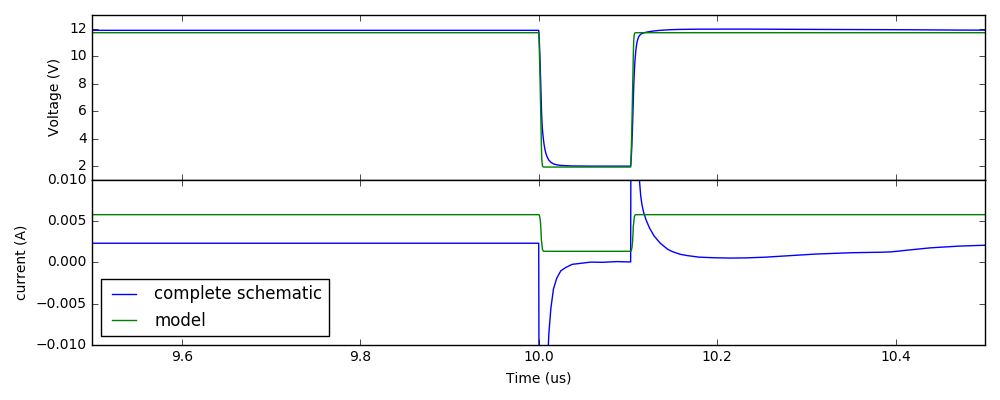
\includegraphics[width=\textwidth]{src/1/figures/comparison_model_total_m10V.png}
  \caption{Comparison of complete schematic and model simulations - -10V TLP}
  \label{fig:compare-model-simu-m10}
\end{figure}

% Check the output
La même vérification est effectuée pour la sortie.
Le cas de la broche de sortie est plus complexe, car contrairement à l'entrée celle-ci doit délivrer un courant statique et ne s'apparente pas à une impédance passive.
Pour reproduire ce comportement, un premier modèle est proposé Fig. \ref{fig:first-output-model}.

\begin{figure}[!h]
  \centering
  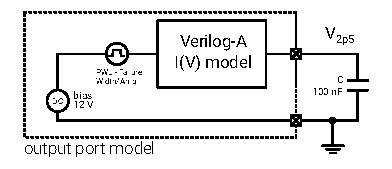
\includegraphics[width=0.3\textwidth]{src/1/figures/first_output_model.png}
  \caption{First proposal for modeling function output}
  \label{fig:first-output-model}
\end{figure}

% Is this first model working
Les premiers tests montrent que cette approche ne fonctionne pas.
Le modèle de la sortie échoue à reproduire le courant en statique uniquement avec la courbe I(V) du TLP, et n'est pas suffisamment précise pour reproduire l'amplitude de la perturbation sur la sortie.
Par ailleurs, ce modèle requiert en plus de prendre en compte le niveau sur l'entrée et de changer de comportement en cas de faute.
Cela apelle probablement à un modèle de sortie controllé par l'entrée, en plus des contraintes existantes pour le faire fonctionner en nominal.
Tous ces problèmes seront étudiés dans des travaux futurs afin d'être capable de proposer un modèle fonctionnel, pouvant servir pendant les phases de conception des cartes électroniques.

% Conclusion
En conclusion, les modèles boite-noire sont une solution intéressante pour représenter le comportement d'une fonction intégré et pouvoir la distribuer sans révéler d'informations sensibles.
L'objectif s'intègre bien avec la méthodologie SEED (System-level ESD Efficient Design) qui préconise de distribuer la responsabilité de la protection face aux ESD entre les circuits intégrés et les cartes électroniques.
Concrètement, cela se traduit par protéger le circuit à tous les niveaux, avec des composants externes, internes, et en s'assurant que ces composants travaillent efficacement ensemble.
Dans la première partie de ce chapitre, une méthode d'extraction de modèle de faute a été présentée.
Elle permet de créer des modèles boite-noire de la faute d'une fonction entre une entrée et une sortie.
Il y a énormément de possibilités d'expérimentation, et la méthode n'en est qu'à ses balbutiements, mais le concept de base semble efficace.
La seconde partie de la méthode consiste à modéliser et simplifier les entrées et sortie électriquement par d'une charactérisation TLP.
L'objectif est de réduire la complexité et les temps de simulation.
Cette méthode s'est avérée fonctionnelle pour la modélisation d'une entrée, mais ne fonctionne pas pour une sortie qui doit fournir du courant.
Des travaux et des investigations supplémentaires sont requises pour corriger ces problèmes.

% Opening work
Il y a énormément de pistes de recherche sur la modélisation boite-noire pour l'ESD.
Le comportement de ces modèles face à des impulsions plus variables tels que des décharges de pistolet ESD doit être étudié.
Ensuite, la modélisation par droite linéaire par morceaux a besoin d'être améliorée afin d'être plus précise vis-à-vis de la courbe I(V) originale.
La méthode présentée doit être testée sur un plus grand nombre de fonctions analogiques, afin de voir si elle peut être appliquée généralement.
